\documentclass[12pt,titlepage]{article}
\usepackage[margin=1.25in]{geometry}
\usepackage{graphicx,amsmath,enumitem,minted}

%% Variables definition
\newcommand{\vSubject}{Data Structure and Algorithm Practicum}
\newcommand{\vSubtitle}{Binary Tree}
\newcommand{\vName}{Dicha Zelianivan Arkana}
\newcommand{\vNIM}{2241720002}
\newcommand{\vClass}{1i}
\newcommand{\vDepartment}{Information Technology}
\newcommand{\vStudyProgram}{D4 Informatics Engineering}

%% [START] Tikz related stuff
\usepackage{tikz}
\usetikzlibrary{svg.path,calc,shapes.geometric,shapes.misc}
\tikzstyle{terminator} = [rectangle, draw, text centered, rounded corners = 1em, minimum height=2em]
\tikzstyle{preparation} = [chamfered rectangle, chamfered rectangle sep=0.75em, draw, text centered, minimum height = 2em]
\tikzstyle{process} = [rectangle, draw, text centered, minimum height=2em]
\tikzstyle{decision} = [diamond, aspect=2, draw, text centered, minimum height=2em]
\tikzstyle{data}=[trapezium, draw, text centered, trapezium left angle=60, trapezium right angle=120, minimum height=2em]
\tikzstyle{connector} = [line width=0.25mm,->]
%% [END] Tikz related stuff

%% [START] Fancy header related stuff
\usepackage{fancyhdr}
\pagestyle{fancy}
\setlength{\headheight}{15pt} % compensate fancyhdr style
\fancyhead{}
\fancyfoot{}
\fancyfoot[L]{\thepage}
\fancyfoot[R]{\textit{\vSubject - \vSubtitle}}
\renewcommand{\footrulewidth}{0.4pt}% default is 0pt, overline for footer
%% [END] Fancy header related stuff

%% [START] Custom tabular command related stuff
\usepackage{tabularx}
\newcommand{\details}[2]{
    #1 & #2  \\
}
%% [END] Custom tabular command related stuff

%% [START] Figure related stuff
\newcommand{\image}[3][1]{
    \begin{figure}[h]
        \centering
        \includegraphics[#1]{#2}
        \caption{#3}
        \label{#3}
    \end{figure}
}
%% [END] Figure related stuff

\begin{document}
\begin{titlepage}
    \centering
    \vfill
    {\bfseries\LARGE
        \vSubject\\
        \vskip0.25cm
        \vSubtitle
    }
    \vfill
    
\includegraphics[width=6cm]{images/polinema-logo.png}
    \vfill
    {
        \textbf{Name}\\
        \vName\\
        \vskip0.5cm
        \textbf{NIM}\\
        \vNIM\\
        \vskip0.5cm
        \textbf{Class}\\
        \vClass\\
        \vskip0.5cm
        \textbf{Department}\\
        \vDepartment\\
        \vskip0.5cm
        \textbf{Study Program}\\
        \vStudyProgram
    }
\end{titlepage}

\section{Questions}
\begin{enumerate}
    \item {
        Why the data searching process is more efficient in the binary search tree than in ordinary binary tree?

        Because in binary search tree, the data is already sorted, which means we can apply the binary search algorithm throughout the binary tree.
        Unlike an ordinary binary tree which may not be sorted so we can't apply the binary search algorithm to the data.
    }
    \item {
        Why do we need the \textbf{Node} class? What are the \textbf{left} and \textbf{right} attributes?

        The \texttt{Node} class represents the node inside the tree that contains the data.
        The \texttt{left} and \texttt{right} attribute represents the left and right child of the node. Since this is a binary tree,
        there would only be 2 child nodes.
    }
    \item {
        \begin{enumerate}[label=\alph*.)]
            \item {
                What are the uses of the \textbf{root} attribute in \texttt{BinaryTree} class?

                It is used so that we can keep track of the root of the tree.
            }
            \item {
                When the tree object was first created, what is the value of \textbf{root}?

                The root of the tree is set to be \texttt{null} at first because it doesn't contain anything
            }
        \end{enumerate}
    }
    \item {
        When the tree is still empty, and a new node is added, what process will happen?

        The newly added node will be assigned as a root because the tree is empty which means that it has no root yet.
    }
    \item {
        Pay attention to the \texttt{add()} method, in which there are program lines as below. 
        Explain in detail what the program line is for?

        \begin{minted}[autogobble,fontsize=\small]{java}
            if (data < current.data) {
                if (current.left != null) {
                    current = current.left;
                } else {
                    current.left = new Node(data);
                    break;
                }
            }
        \end{minted}

        It checks if the data that we want to insert is less than the current node that we're in. If so, then we'll go to the left by assigning the current left node into current itself.
        This will make it so that we traverse to the left of the current node. When we reach a condition where the current data is greater than the current node data, then we'll assign it
        as its left child node.
    }
    \pagebreak
    \item {
        What is the difference between pre-order, in-order, and post-order traverse modes?

        \begin{itemize}
            \item {
                \textbf{pre-order}
                pre-order traversal of the tree starts from the root node and then traverses the left subtree, then traverses the right subtree.
                It goes from root -> left -> right
            }
            \item {
                \textbf{in-order}
                in-order traversal of the tree starts from the root node and then traverses the left subtree, then traverses the root node, then traverses the right subtree.
                It goes from left -> root -> right
            }
            \item {
                \textbf{post-order}
                post-order traversal of the tree starts from the root node and then traverses the left subtree, then traverses the right subtree, then traverses the root node.
                It goes from left -> right -> root
            }
        \end{itemize}
    }
    \item {
        Look at the \texttt{delete()} method. Before the node removal process, it is preceeded by the process of finding the node to be deleted.
        Besides intended to find the node to be deleted (current), the search process will also look for the parent of the node to be deleted (parent).
        In your opinion, why is it necessary to know the parent of the left node to be deleted?

        We need to know the parent of the left node to be deleted because we want to re-connect the left child into its parent.
        If we don't connect the node after removing it, then the tree starting from the one we remove will be broken / disconnected from the rest of the tree.
    }
    \item {
        For what is a variable named \texttt{isLeftChild} created in the \texttt{delete()} method?

        It is used to check if the current node is a left child.
    }
    \item {
        What is the \texttt{getSuccessor()} method for?

        It is used to find the successor of the current node in the binary tree.
    }
    \item {
        In a theoritical view, it is stated that when a node has 2 children is deleted, the node is replaced by the successor node, where the successor node
        can be obtained in 2 ways, namely:
        \begin{enumerate}
            \item Looking for the largest value of the subtree to the left, or
            \item Looking for the smallest value of the subtree on the right.
        \end{enumerate}
        Which 1 of 2 methods is implemented in the \texttt{getSuccessor()} method in the above program?

        It looks for the largest value of the subtree to the left. This is determined by the \texttt{successfor.left != null} which means it will try to traverse
        the left path until there is no left child node left, effectively finding the largest value of the subtree to the left.
    }
    \item {
        What are the uses of the data and \texttt{idxLast} attributes in the \texttt{BinaryTreeArray} class?

        It is used so that we can keep track of the last index of the array that contains the tree.
    }
    \item {
        What are the uses of the \texttt{populateData()} and \texttt{traverseInOrder()} methods?

        \begin{itemize}
            \item \texttt{populateData}: used to populate the data inside the \texttt{BinaryTreeArray} class
            \item \texttt{traverseInOrder}: used to traverse the data inside the \texttt{BinaryTreeArray} class
        \end{itemize}
    }
    \item {
        If a binary tree node is stored in index array 2, when in what index are the left-child and right-child position respectively?

        The left child will be positioned in $n * 2 + 1$ and the right child will be positioned in $n * 2 + 2$ where n is the index of the node.
        In this case it's 2, so that means the left child will be positioned at index 5 and the right child will be positioned at index 6.
    }
\end{enumerate}

\pagebreak

\section{Assignments}
\begin{enumerate}
    \item {
        Create a method inside the \texttt{BinaryTree} class that will add nodes with recursive approach!

        \begin{minted}[autogobble,fontsize=\small]{java}
            void recursiveAdd(int data) {
                recursiveAdd(data, root);
            }

            void recursiveAdd(int data, Node parent) {
                if (isEmpty()) {
                    root = new Node(data);
                    return;
                }
                if (data < parent.data) {
                    if (parent.left != null) {
                        recursiveAdd(data, parent.left);
                    } else {
                        parent.left = new Node(data);
                    }
                } else if (data > parent.data) {
                    if (parent.right != null) {
                        recursiveAdd(data, parent.right);
                    } else {
                        parent.right = new Node(data);
                    }
                }
            }
        \end{minted}
    }
    \pagebreak
    \item {
        Create a method inside the \texttt{BinaryTree} class to display the smallest and largest value in the tree!

        \begin{minted}[autogobble,fontsize=\small]{java}
            void displayLargestAndSmallest() {
                int smallest = Integer.MAX_VALUE;
                int largest = Integer.MIN_VALUE;

                // traverse the left part to find the smallest value
                Node current = root;
                while (current != null) {
                    if (current.data < smallest) {
                        smallest = current.data;
                    }
                    current = current.left;
                }

                // traverse the right part to find the largest value
                current = root;
                while (current != null) {
                    if (current.data > largest) {
                        largest = current.data;
                    }
                    current = current.right;
                }

                System.out.println("Smallest: " + smallest);
                System.out.println("Largest: " + largest);
            }
        \end{minted}
    }
    \item {
        Create a method in the \texttt{BinaryTree} class to display the data in the leaf!

        \begin{minted}[autogobble,fontsize=\small]{java}
            void displayLeafData(Node node) {
                if (node == null) return;
                if (node.left == null && node.right == null) {
                    System.out.print(node.data + " ");
                    return;
                }
                displayLeafData(node.left);
                displayLeafData(node.right);
            }
        \end{minted}
    }
    \pagebreak
    \item {
        Create a method in the \texttt{BinaryTree} class to display the number of leaves in the tree!

        \begin{minted}[autogobble,fontsize=\small]{java}
            int countLeaves(int count, Node node) {
                if (node == null) return 0;
                if (node.left == null && node.right == null) return count + 1;
                return countLeaves(count, node.left) + countLeaves(count, node.right);
            }
        \end{minted}
    }
    \item {
        Modify the \texttt{BinaryTreeMain} class, so that it has a menu option:
        \begin{enumerate}[label=\alph*.)]
            \item \texttt{add}
            \item \texttt{delete}
            \item \texttt{find}
            \item \texttt{traverseInOrder}
            \item \texttt{traversePreOrder}
            \item \texttt{traversePostOrder}
            \item \texttt{exit}
        \end{enumerate}

        \begin{minted}[autogobble,fontsize=\small]{java}
            public class BinaryTreeMain {
                public static void main(String[] args) {
                    Scanner scanner = new Scanner(System.in);
                    BinaryTree binaryTree = new BinaryTree();

                    while (true) {
                        showMenu();
                        System.out.print("Enter your choice: ");
                        int chosenMenu = scanner.nextInt();
                        switch (chosenMenu) {
                            case 1:
                                System.out.print("Insert the value: ");
                                int valueAdded = scanner.nextInt();
                                binaryTree.add(valueAdded);
                                break;
                            case 2:
                                System.out.print("Delete the value: ");
                                int valueDeleted = scanner.nextInt();
                                binaryTree.delete(valueDeleted);
                                break;
                            case 3:
                                System.out.print("Find the value: ");
                                int valueSearch = scanner.nextInt();
                                boolean found= binaryTree.find(valueSearch);
                                System.out.println(found ? "Found" : "Not Found");
                                break;
                            case 4:
                                binaryTree.traverseInOrder(binaryTree.root);
                                System.out.println();
                                break;
                            case 5:
                                binaryTree.traversePreOrder(binaryTree.root);
                                System.out.println();
                                break;
                            case 6:
                                binaryTree.traversePostOrder(binaryTree.root);
                                System.out.println();
                                break;
                            case 7:
                                System.out.println("Bye!");
                                return;
                        }
                    }
                }

                static void showMenu() {
                    System.out.println("Menu");
                    System.out.println("1. Add");
                    System.out.println("2. Delete");
                    System.out.println("3. Find");
                    System.out.println("4. Traverse In Order");
                    System.out.println("5. Traverse Pre Order");
                    System.out.println("6. Traverse Post Order");
                    System.out.println("7. Exit");
                }
            }
        \end{minted}

        \pagebreak

        \begin{figure}[h]
            \centering
            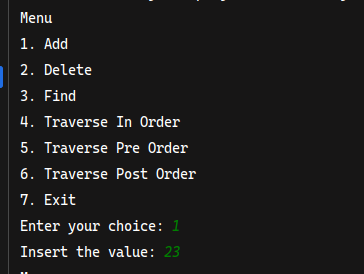
\includegraphics[width=.5\textwidth]{./images/a.png}
            \caption{Add}
        \end{figure}
        \begin{figure}[h]
            \centering
            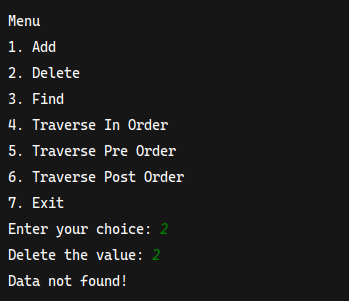
\includegraphics[width=.5\textwidth]{./images/b.png}
            \caption{Delete}
        \end{figure}
        \pagebreak
        \begin{figure}[h]
            \centering
            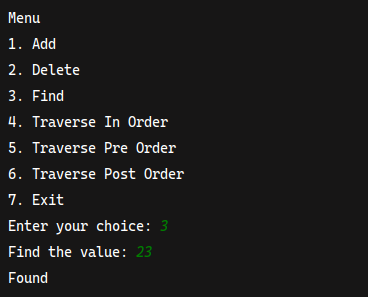
\includegraphics[width=.5\textwidth]{./images/c.png}
            \caption{Find}
        \end{figure}
        \begin{figure}[h]
            \centering
            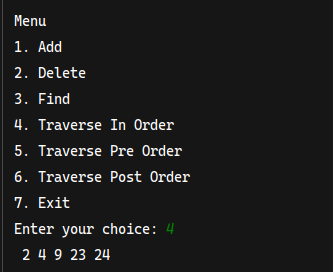
\includegraphics[width=.5\textwidth]{./images/d.png}
            \caption{Traverse In Order}
        \end{figure}
        \pagebreak
        \begin{figure}[h]
            \centering
            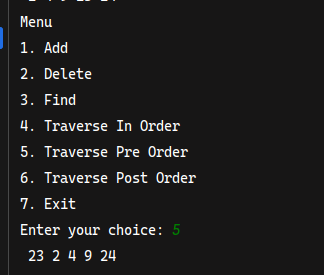
\includegraphics[width=.5\textwidth]{./images/e.png}
            \caption{Traverse Pre Order}
        \end{figure}
        \begin{figure}[h]
            \centering
            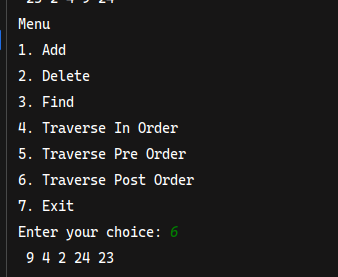
\includegraphics[width=.5\textwidth]{./images/f.png}
            \caption{Traverse Post Order}
        \end{figure}
        \pagebreak
        \begin{figure}[h]
            \centering
            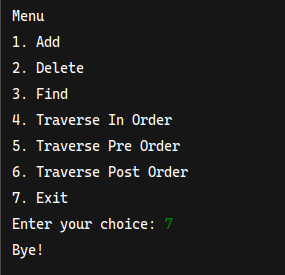
\includegraphics[width=.5\textwidth]{./images/g.png}
            \caption{Exit}
        \end{figure}
    }
    \pagebreak
    \item {
        Modify the \texttt{BinaryTreeArray} class and add:
        \begin{enumerate}[label=\alph*.)]
            \item{
                Add a method \texttt{add(int data)} to enter data into the tree

                \begin{minted}[autogobble,fontsize=\small]{java}
                    void add(int data) {
                        int currentIdx = 0;
                        while (true) {
                            if (currentIdx >= idxLast) {
                                break;
                            }
                            if (data > this.data[currentIdx]) {
                                currentIdx = currentIdx * 2 + 2;
                            } else if (data < this.data[currentIdx]) {
                                currentIdx = currentIdx * 2 + 1;
                            } else {
                                break;
                            }
                        }
                        this.data[currentIdx] = data;
                    }
                \end{minted}
            }
            \item {
                \texttt{traversePreOrder()} and \texttt{traversePostOrder} methods

                \begin{minted}[autogobble,fontsize=\small]{java}
                    void traversePreOrder(int idxStart) {
                        if (idxStart <= idxLast) {
                            System.out.print(data[idxStart] + " ");
                            traversePreOrder(idxStart * 2 + 1);
                            traversePreOrder(idxStart * 2 + 2);
                        }
                    }

                    void traversePostOrder(int idxStart) {
                        if (idxStart <= idxLast) {
                            traversePostOrder(idxStart * 2 + 1);
                            traversePostOrder(idxStart * 2 + 2);
                            System.out.print(data[idxStart] + " ");
                        }
                    }
                \end{minted}
            }
        \end{enumerate}
    }
\end{enumerate}

\end{document}

